\chapter*{Introducción*}
En el núcleo del método científico se encuentra la interacción entre la teoría y el experimento: la formulación de una hipótesis y la prueba de dicha hipótesis a través de la experimentación, permitieno que la física de altas energías se encuentre en una situación peculiar después del descubrimiento del bosón de Higgs en 2012, el Modelo estándar de física de partículas se ha completado, pero a pesar de sus muchos éxitos, el Modelo Estándar no puede dar cuenta de muchos fenómenos que observamos, como la existencia de Dark Matter, la asimetría de materia-antimateria o el origen de las masas de neutrinos, entre otros. En las últimas décadas, se han propuesto muchas nuevas teorías para explicar estos fenómenos, pero a menudo solo se pueden probar utilizando los datos de los pocos experimentos del Gran Colisionador de Hadrones, ya que nos permiten recrear escenarios que de otra forma no podrían ser estudiados. 

Probar una teoría implica una medición cuidadosa de las colisiones en un subconjunto particular de la población de datos. Los equipos de análisis deben calcular con precisión cuántos eventos se esperarían de los procesos del Modelo Estándar en ese subconjunto y, de manera similar, cuántos eventos cabría esperar de la teoría particular de la nueva física en la que uno está interesado. Con estos cálculos en mano, los analistas pueden mirar los datos reales observados y realizar un análisis estadístico que indicara si la teoría particular es favorecida por los datos, normalmente dicho análisis se define mediante un complejo análisis basada en software. La mayor parte del trabajo en el desarrollo de un teoría consiste en crear un respaldo en datos que contiene la mayor cantidad de información sobre la teoría estudiada, así como también en hacer los cálculos precisos del Modelo Estándar.
Esto es especialmente importante dada la gran variedad de posibles teorías de la nueva física. Aquí se puede emplear un método poderoso: la reinterpretación.

La reinterpretación explota el hecho de que los efectos de una teoría pueden materializarse en un subconjunto de la población de datos que ya se analizó con respecto a una teoría diferente, si es el caso, el segmento de datos y el código para analizar están bien definidos, el próximo paso es calcular la estimación del efecto de la nueva teoría y realizar el análisis estadístico para decidir si es viable frente a los datos observados o no.







%Partiendo del supuesto que la materia oscura está compuesta de partículas elementales las cuales pueden ser producidas en los laboratorios modernos de física de partículas. De ser esto cierto se requiere de un nuevo marco teórico, una extensión al modelo estándar que sustente dicha hipótesis y el modelo conocido como "dark SUSY"~\cite{susy} en el cual predice un llamado sector oscuro donde por medio del rompimiento del grupo de simetría $U(1)_{D}$ se da lugar a la creación de fotones oscuros ($\gamma_{D}$) ligeros, los cuales interactuarían con partículas del modelo estándar y dicha fuerza de interacción estaría descrita por medio de un parámetro de mezcla cinético $\epsilon$.  Una representación gráfica entre el sector oscuro y el del modelo estándar representa en la la Figura~\ref{fig:sketch_darksector} (izquierda). En "dark SUSY" además de partículas de materia oscura se da lugar a la producción de partículas supersimétricas (SUSY), en donde la mas ligera de estas, el neutralino, dejarían de ser estable y podría decaer al fotón oscuro. 
%
%Las nuevas fuerzas en "dark SUSY" estarían mediadas mediante un término de acoplamiento a la hipercarga del modelo estándar, descrito por la lagrangiana \cite{bb38,bb39}.
%
%\begin{equation} 
%L_{KM} = \frac{\epsilon}{2} F_{\mu\nu}^{\gamma}F^{D_{\mu\nu}}
%\end{equation}
%
%Donde $F_{\mu\nu}^{D}$ representa el campo oscuro y $\epsilon$ es un parámetro constante relacionado con la interacción.  De esta manera se obtiene como el fotón oscuro puede decaer a leptones \cite{bb41} del modelo estándar con una amplitud de decaimiento dada por:
%
%\begin{equation}
%  \Gamma_{\gamma D \rightarrow ll} = \frac{1}{3}\alpha \epsilon^{2} m_{\gamma D} \sqrt{1-\frac{4 m_{l}^{2}}{m_{\gamma D}^2}}(1+\frac{2m_{l}^{2}}{m_{\gamma D}}^{2})
%\end{equation}
%
%La expresión para las amplitudes permite calcular el tiempo de vida del fotos oscuro dado por: 
%
%\begin{equation}
%  \tau_{\gamma D}= \frac{\hbar}{\Gamma_{\gamma D Total}}=\frac{1}{\Gamma_{\gamma D \rightarrow e^{+}e^{-}}  + \Gamma_{\gamma D \rightarrow \mu^{+}\mu^{-}} + \Gamma_{\gamma D \rightarrow hadrons}}
%\end{equation}
%
%%%% EScribir la ecuacion. 
%
%%%JUSTIFICACION
%
%Los estudios de nueva física, en particular los que predicen la producción de nuevas partículas, son bastantes relevantes dado que se aproxima la etapa de alta luminosidad del Gran Colisionador de Hadrones en donde se logrará acumular datos con una frecuencia 10 veces mayor en la que se estaba operando. Lo anterior indica que la probabilidad de detección de nuevas señales será mucho mayor ya que se logrará alcanzar un rango de energía mayor y una cantidad de datos igualmente superior. Usualmente la probabilidad de producción de estas partículas exóticas es baja por lo que se requiere de una cantidad grande de datos para poder observar dicha producción. El período de alta luminosidad está programado para empezar a partir del año 2024 o 2025, como se puede ver en al línea de tiempo del Gran Acelerador de Hadrones en la Figura \ref{fig:LHC_timeline}, sin embargo desde este momento se está trabajando en la actualización del detector, en métodos de análisis y en estrategias que ayuden a optimizar la búsqueda de nueva física.
%
%\begin{figure}
%    \centering
%    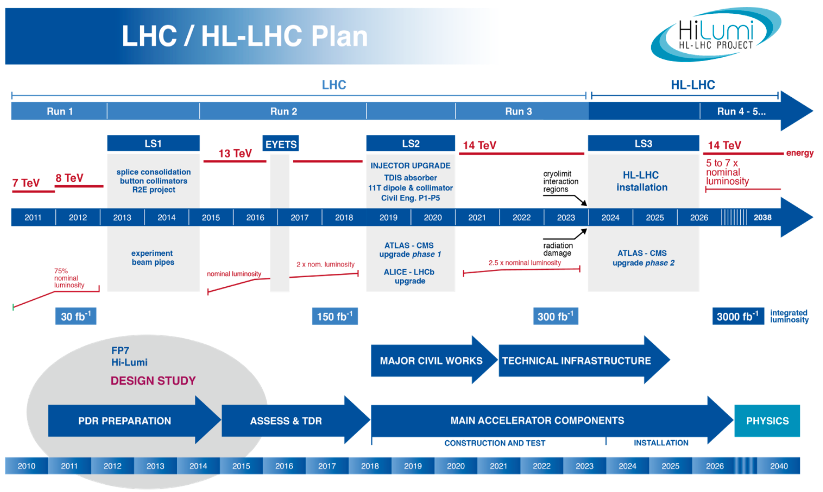
\includegraphics[width=0.84\textwidth]{Introduccion/imagenes/LHC_timeline.png}
%    \caption{Agenda de actividades del Gran Colisionador de Hadrones, donde la fase de alta luminosidad está programada para iniciar a partir del 2024-2025.}
%    \label{fig:LHC_timeline}
%\end{figure}
%
%Actualmente los modelos teóricos que predicen la formación de partículas de materia oscura no han sido explorados ampliamente, en gran medida por falta de datos experimentales que permitan alcanzar el espacio fase que dichos modelos predicen para esas partículas. Por todo ello el funcionamiento del Gran Acelerador de Hadrones y sus proyecciones en cuanto a recolección de datos en los próximos años constituye una oportunidad perfecta para explotar con mayor intencionalidad el estudio de dichos modelos en aras de descubrir una nueva señal de fácil interpretación en el contexto de los modelos propuestos. 
%
%
%
%
%%% PROPUESTA
%El diagrama de Feynman para el proceso del modelo "dark SUSY" $h\rightarrow 2n_{1}\rightarrow 2n_{D}\rightarrow 2\gamma_{D} \rightarrow 2n_{D} + 4\mu$ se muestra en la figura~\ref{fig:sketch_darksector} (derecha), el estudio de este proceso y la obtención de sus características (ver Figura \ref{fig:foton_oscuro}) permitiría inicializar escenarios extendidos de "dark SUSY" para estudios con versiones mas complejas que involucrarían otras partículas del sector oscuro como Higgs oscuros, o bosones Z y W oscuros, dando cabida a procesos como $pp\rightarrow h \rightarrow Z_{D}Z/Z_{D}Z_{D}/Z_{a}\rightarrow 4\mu$. %Sin embargo dichos modelos escapan a los alcances de esta tesis y podran ser explorados en un analsis futuro. 
%
%%Este escenario simple "dark SUSY" podria ser extendido de diversas maneras para estudios posteriores, como por ejemplo, en versiones mas complejas que involucrarían otras partículas del sector oscuro como Higgs oscuros, o bosones Z y W oscuros, dando cabida a procesos como $pp\rightarrow h \rightarrow Z_{D}Z/Z_{D}Z_{D}/Z_{a}\rightarrow 4\mu$. %Sin embargo dichos modelos escapan a los alcances de esta tesis y podrian ser explorados en un analsis futuro. 
%
%\begin{figure}[h]
%    \centering
%   % 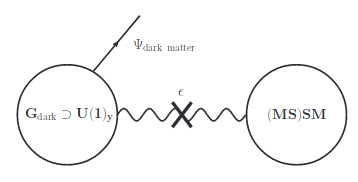
\includegraphics[width=0.4\textwidth]{HIPOTESIS/sketch_darksector.png}
%    %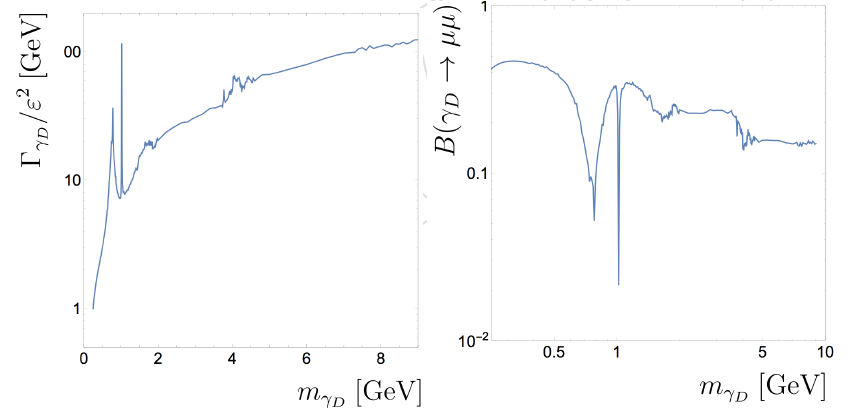
\includegraphics[width=0.8\textwidth]{imagenes/foton_oscuro.png}
%    \caption{Izquierda: Peso total de los diferentes modos de desintegración del fotón oscuro, normalizado por $\epsilon^2$. Derecha: Probabilidad de 			             decaimiento para $\gamma_D = \mu \mu$.}
%    \label{fig:foton_oscuro}
%\end{figure}
%
%Entonces si se propone hacer un estudio, por medio de simulación de Monte Carlo, de un modelo teórico que predice la creación de nuevas partículas como producto de la colisión de protones altamente energéticos. Estas nuevas partículas serían candidatos a explicar la composición de la materia oscura. Usualmente en dichos modelos las nuevas partEn una primera fase se pretende analizar los modelos teóricos de una manera fenomenológica, es decir por medio de paquetes de simulación propios del área de altas energías, en los cuales se pretende entender los principios básicos del formalismo de altas energías, lo cual incluye los lagrangianos, diagramas de feynman, reglas de decaimientos. En un segundo paso se pretende simular la respuesta del detector a las nuevas señales buscando optimizar la selección de los eventos en base a las propiedades de cada modelo. En una tercera fase se pretende estudiar la señal de dichos modelos bajo diferentes escenarios del detector CMS, un primer escenario sería usando en simulación la configuración actual del detector CMS, es decir la geometría, materiales y dimensiones con la cual opera actualmente el detector (configuración usada hasta el 2018), durante el llamado período 'Run-2' y comparar los resultados con el detector que se tiene propuesto para la fase de alta luminosidad o también llamada Phase-2, la cual empezará a partir del 2025; de esta manera se puede predecir en base a los estudios de simulación las posibilidades de identificación de una nueva señal en los próximos años y cómo la actualización de los detectores y métodos de identificación de partículas podrían contribuir a incrementar las probabilidades de descubrimiento de estas nuevas partículas.
%
%ículas interaccionan débilmente con las partículas del modelo estándar, es decir con la materia visible, por lo que su detección se dará de forma indirecta, o en otras palabras, por su decaimiento a partículas conocidas del modelo estándar~\cite{Curtin2015}. Adicionalmente al estudio del modelo teórico se pretende trabajar en la parte experimental, la cual consiste en el estudio de la respuesta del detector al paso de las nuevas partículas y de esta manera extraer observables experimentales como son la energía de las partículas, el momento y la trayectoria, eficiencia de identificación, resoluciones, entre otros que permitan distinguir el proceso de se\~nal de los procesos de ruido. La parte experimental es fundamental ya que sin una buena estrategia de selección de datos, técnicas de supresión de ruido y optimización de la señal sería imposible la observación de nueva física. En este proyecto se considera el detector CMS del CERN como el aparato experimental que proporcionará los datos de estudio, ya sea por simulación o por uso de datos reales.
%
%
%%% METODOLOGIA
%
%%{\let\clearpage\relax\chapter{Metodología}}
%
%Con el fin de alcanzar los objetivos planteados se plantea la siguiente secuencia de actividades:
%
%
%\begin{itemize}
%    \item Producción de muestras de Monte Carlo (2 meses): Se espera implementar el modelo "dark SUSY" usando los paquetes propios del área y producir muestras de simulación para el proceso de señal. Las muestras se producirán usando los recursos computacionales de la Universidad de Sonora. Este paso requiere del desarrollo de código para la distribución de las corridas de simulación en forma paralela usando el cluster ACARUS. Los paquetes de simulación que se usarán serán FeynRules, MADGRAPH \cite{Alwall:2007st}, Pythia y Delphes \cite{deFavereau2014}.
%    \item Análisis preliminar (2 meses): El estudiante debe desarrollar diferentes herramientas de análisis de datos con el fin de acceder a los datos producidos en la simulación y extraer las variables de interés como lo son las propiedades del fotón oscura (masa, tiempo de vida, etc.). Comúnmente dichas herramientas de análisis consisten en códigos escritos en lenguaje C++ y python, de esta manera el estudiante desarrollará habilidad en la manipulación de muestras de datos.
%    \item Optimización de la selección de eventos (2 meses): Después del acceso de datos de simulación y variables de interés se procederá al estudio de la selección de eventos, la cual a grandes rasgos consiste en seleccionar el conjunto de variables físicas y valores que puedan optimizar el proceso de señal y reducir lo más posible la contribución del ruido.
%    \item Análisis estadístico (3 meses): Se realizará un estudio estadístico en el cual se extraerán el número de eventos de señal y ruido después de la selección. De ahí se puede interpretar los resultados en base a indicadores estadísticos y concluir la probabilidad de observación con datos recolectados en los próximos años.
%    \item Comparación de los resultados obtenidos usando la configuración actual del detector CMS y la configuración que se utilizara en la llamada fase-2 o de alta luminosidad. 
%    \item Escritura de Tesis (3 meses): Se presentará los resultados a expertos del área buscando una retroalimentación, procediéndose al mismo a la escritura del trabajo de tesis.
%\end{itemize}
%
%
%
%%% 
%
%
%
%
%
%
%
%
%
%
%
%
%
%
%
%
%
%
%
